\documentclass{VUMIFInfBakalaurinis}
\usepackage{algorithmicx}
\usepackage{algorithm}
\usepackage{algpseudocode}
\usepackage{amsfonts}
\usepackage{amsmath}
\usepackage{bm}
\usepackage{caption}
\usepackage{color}
\usepackage{float}
\usepackage{graphicx}
% \usepackage{hyperref}  % Nuorodų aktyvavimas
\usepackage{listings}
\usepackage{subfig}
\usepackage{url}
\usepackage{wrapfig}


% Titulinio aprašas
\university{Vilniaus universitetas}
\faculty{Matematikos ir informatikos fakultetas}
\department{Informatikos katedra}
\papertype{Baigiamasis bakalauro darbas}
\title{Algoritmas, maksimaliam srautui dinaminiuose tinkluose rasti}
\titleineng{Algorithm for the maximal flow in dynamic networks}
\status{4 kurso 2 grupės studentas}
\author{Aleksas Vaitulevičius}
\supervisor{lekt. Irmantas Radavičius}
\reviewer{doc. dr. Vardauskas Pavardauskas}
\date{Vilnius \\ \the\year}

% Nustatymai
% \setmainfont{Palemonas}   % Pakeisti teksto šriftą į Palemonas (turi būti įdiegtas sistemoje)
\bibliography{bibliografija.bib} 

\begin{document}
\maketitle


\sectionnonum{Santrauka}
Paskutiniuose dviejuose dešimtmečiuose yra plačiai domimasi dinaminiais grafais, dėl jų naudos tokiose srityse kaip: komunikacijos tinkluose, VLSI kūrime, kompiuterinėje grafikoje. Šis darbas apima dinaminių grafų problemą, maksimalaus srauto radimą,viena iš labiausiai fundamentalių optimizavimo problemų. Šio darbo tikslas yra įrodyti, kad pateikiamo maksimalaus srauto radimo algoritmas yra efektyvesnis už statinio grafo Fordo Fulkersono algoritmą skaičiavimui panaudojamų briaunų atžvilgiu. Pateikiamo algoritmo veikimas yra pagrįstas modifikuotu grupavimo metodu ir modifikuotu Fordo Fulkersono algoritmu. Grupavimo metodas yra skirtas grafo išskirstymui į grupes, o modifikuotas Fordo Fulkersono algoritmas yra skirtas apskaičiuoti konkretaus regiono maksimaliems srautams. Atmintyje bus saugomas regionų išsidėstymas ir jų talpas grafo pavidale. Perskaičiavus grupes kuriuose įvyko pokytis, galima rasti pakitusio grafo maksimalų srautą. \\
Raktažodžiai: dinaminiai grafai, maksimalūs srautai,grupavimo metodas, Fordo Fulkersono algoritmas, euristiniai bandymai.


\sectionnonum{Summary}
In the last two decades, there was a growing interest in dynamical graphs, because of their use in such fields like: communication network, VLSI design, graphics. This work is only about dynamical graph problem, maximum flow, one of the most fundamental optimization problems. The main task of this work is to prove that provided algorithm for solving maximum flow problem is more efficient than Ford Fulkerson algorithm for static graph in the context of used edges for calculation. This algorithm is based on modified clustering method and modified Ford Fulkerson algorithm. Clustering method is used for clustering graph into clusters and modified Ford Fulkerson algorithm is used for computing maximum flows in particular cluster. Positioning and capacity of clusters will be saved in memory. Once updated clusters are computed, it is possible to find maximum flow for the whole updated graph. \\
Keywords: dynamic graphs, max flow, clustering, Ford Fulkerson algorithm, heuristic experiments.

\tableofcontents

\sectionnonum{Sąvokų apibrėžimai}
\begin{enumerate}
	\item sąvoka - paaiškinimas
\end{enumerate}

\sectionnonum{Įvadas}
Paskutiniuose dviejuose dešimtmečiuose yra plačiai domimasi dinaminiais grafais. Ši sritis suteikia daug teorinių žinių, kurios gali būti pritaikytos optimizuojant tokias sritis kaip: komunikacijos tinklus, VLSI kūrimą, kompiuterinę grafiką, kaip yra teigiama publikacijoje Dynamic graphs  \cite{DynamicGraphs}. Šiame darbe bus tiriamas algoritmas skirtas maksimaliam srautui rasti dinaminiuose tinkluose.

Dinaminis grafas - tai grafas, kuriam yra galima atlikti bent vieną iš šių operacijų:
\begin{itemize}
	\item Pridėjimo
	\begin{itemize}
		\item Pridėti briauną.
		\item Pridėti viršūnę.
	\end{itemize}
	\item Atėmimo
	\begin{itemize}
		\item Atimti briauną.
		\item Atimti viršūnę.
	\end{itemize}
	\item  Papildomos operacijos priklausomai nuo grafo savybių(pavyzdžiui jei grafas yra svorinis, tai jis galėtų turėti papildomą operaciją keisti svorį).
\end{itemize}
Pagal leidžiamas operacijas dinaminiai grafai yra skirstomi į:
\begin{itemize}
	\item dalinai dinaminius grafus, kurie yra skirstomi į:
	\begin{itemize}
		\item inkrementalus - vykdoma tik pridėjimo operacija
		\item dekrementalus - Vykdoma tik atėmimas
	\end{itemize}
	\item  pilnai dinaminius grafus, kuriuose vykdomos visos operacijos.
\end{itemize}
Šiame darbe tiriamas algoritmas yra skirtas spręsti pilnai dinaminio grafo uždavinį.

Visa statinio grafo problemų aibė yra dinaminio grafo problemų poaibis. Tačiau dinaminiame grafo problemos sprendimas gali būti optimizuotas, nes yra daugiau informacijos apie grafą nei statiniame grafe (pavyzdžiui, jei buvo apskaičiuotas grafo maksimalus srautas ir prie grafo buvo pridėta briauna, tai bus žinomas grafo poaibio, kuriam nepriklauso naujai pridėta briauna, maksimalus srautas). Šiame darbe tiriamas algoritmas sprendžia maksimalaus srauto problemą, kuri priklauso šiai aibei.

Maksimalus srautas - tai didžiausias galimas srautas tinkle iš viršūnių $s_i$ (šaltinių) iki viršūnių $t_i$ (tikslų). Tinklas - tai orientuotas grafas $G= {V, E, u}$, kur V yra viršūnių aibė, E - briaunų aibė, o u - briaunų pralaidumų aibė$ ( u : E \rightarrow R )$. Dinaminio tinklo apibrėžimas yra analogiškas dinaminio grafo apibrėžimui. Pagal šaltinių ir tikslų skaičių ši problema yra skirstoma į:
\begin{itemize}
	\item Vienšaltinę daugtikslinę - tai srautas, kuriame yra vienas šaltinis ir daugiau nei vienas tikslas.
	\item Daugiašaltinę vientikslinę - tai srautas, kuriame yra vienas tikslas ir daugiau nei vienas šaltinis.
	\item Daugiašaltinę daugtikslinę - tai srautas, kuriame yra daugiau nei vienas šaltinis ir daugiau nei vienas tikslas.
	\item Vienšaltinę vientikslinę - tai srautas, kuriame yra vienas šaltinis ir vienas tikslas.
\end{itemize}
Algoritmas, tiriamas šiame darbe, sprendžia tik vienšaltinę vientikslinę problemą. Tačiau tarpinėms reikšmėms gauti yra naudojama ir likusių problemų sprendimo būdas, Fordo Fulkersono algoritmas pritaikytas spręsti daugiašaltinę daugtikslinę problemą.

Šiame darbe tiriamas algoritmas yra paremtas Frederiksono suformuluotu grupavimo metodu \cite{DSfUoMST}. Grupavimo metodas - tai metodas, kuris yra pagrįstas grafo dalinimu į subgrafus vadinamus grupėmis. Grafas yra padalinamas taip, kad kiekviena atlikta operacija turėtų įtakos tik daliai grupių, bet ne visoms. Šių grupių maksimaliems srautams rasti yra naudojamas Fordo Fulkersono algoritmas pritaikytas spręsti daugiašaltinę daugtikslinę problemą.

Šiame darbe tiriamo algoritmo korektiškumas nėra įrodytas. Jo veikimo korektiškumą gali pagrįsti tik matematinis įrodymas. Tačiau matematinis įrodymas yra sudėtingas procesas. Tad reikia atlikti empirinius tyrimus su algoritmu, kurie parodytų ar verta tirti algoritmą. Taip pat nėra nustatyta ar tiriamas algoritmas yra efektyvesnis už algoritmą randantį maksimalų srautą statiniame tinkle. Jei tiriamas algoritmas nėra efektyvesnis, tai jo įrodyta neapsimoka, nes algoritmai skirti statiniams grafams, gali būti pritaikyti ir dinaminiams. Tad algoritmai, skirti dinaminiams grafams, yra naudojami tik tuo atveju jei jie yra efektyvesni už algoritmus, skirtus statiniams grafams.

Tad šio darbo \textbf{TIKSLAS} yra įgyvendinti empirinį tyrimą, kuris įrodytų, kad šiame darbe tiriamą algoritmą yra verta matematiškai ištirti. Šiam tikslui pasiekti reikia atlikti šiuos uždavinius:
\begin{enumerate}
	\item Pateikti tiriamą algoritmą:	
	\begin{enumerate}
		\item Pateikti grupės, į kurias bus sugrupuotas grafas, apibrėžimą.
		\item  Pateikti Fordo Fulkersono algoritmą ir kaip jis buvo pritaikytas daugšaltinei daugtikslinei problemai.
		\item Pateikti grupavimo funkciją.
		\item Apibrėžti funkciją, kuri randa viso tinklo maksimalų srautą su pakitusiu bent vienu maksimaliu srautu vienoje ar keliose grupėse. Jei buvo įvykdyta operacija:
		\begin{enumerate}
			\item Pridėti viršūnę
			\item Pridėti briauną
			\item Atimti viršūnę
			\item Atimti briauną
			\item Pakeisti briaunos pralaidumą
		\end{enumerate}
		\item Pateikti tiriamo algoritmo pagrindinę funkciją.
	\end{enumerate}
	\item Pateikti tiriamo algoritmo panaudojimo pavyzdį.
	\item Įgyvendinti tiriamą algoritmą.
	\item Įgyvendinti Fordo Fulkersono algoritmą, skirtą rasti maksimalų srautą statiniame tinkle.
	\item Atlikti empirinius bandymus:
		\begin{enumerate}
			\item Surinkti šiuos duomenis apie tiriamą algoritmą ir įgyvendintą algoritmą, skirtą rasti maksimalų srautą statiniame tinkle:
			\begin{enumerate}
				\item Abiejų algoritmų skaičiavimų rezultatus.
				\item Abiejų algoritmų skaičiavimuose panaudotų briaunų kiekius.
				\item Abiejų algoritmų skaičiavimuose panaudotų viršūnių  kiekius.
			\end{enumerate}
			\item Ištirti koreliaciją tarp briaunų panaudotų skaičiavimuose tiriamo algoritmo ir tinklo, naudojamo skaičiavimuose, briaunų kiekius. 
			\item Ištirti koreliaciją tarp briaunų panaudotų skaičiavimuose tiriamo algoritmo ir tinklo, naudojamo skaičiavimuose, viršūnių kiekius. 
			\item Ištirti koreliaciją tarp briaunų panaudotų skaičiavimuose Fordo Fulkersono algoritmo ir tinklo, naudojamo skaičiavimuose, briaunų kiekius. 
			\item Ištirti koreliaciją tarp briaunų panaudotų skaičiavimuose Fordo Fulkersono algoritmo ir tinklo, naudojamo skaičiavimuose, viršūnių kiekius. 
			\item Palyginti tiriamo algoritmo ir Fordo Fulkersono algoritmo rezultatus.
			\item Palyginti tiriamo algoritmo ir Fordo Fulkersono algoritmo koreliacijas.
	\end{enumerate}
\end{enumerate}

Darbas susideda iš dviejų dėstymo skyrių. Pirmame skyriuje yra pateikiamas tiriamas algoritmas. Pirmo skyriaus pirmame poskyryje yra pateikiamas grupės apibrėžimas, tam, kad žinoti į kokius subgrafus bus skaidomi tinklai tiriamame algoritme. Antrame poskyryje yra pateikiamas Fordo Fulkersono algoritmas ir kaip jis buvo pritaikytas maksimaliems srautams rasti grupėse. Trečiame poskyryje pateikiama grupavimo funkcija. Ketvirtas poskyris yra skirtas pateikti visoms funkcijoms, kurios būna iškviečiamos  atlikus pridėjimo, atėmimo arba briaunos pralaidumo pakeitimo operacijas. Paskutiniame poskyryje pirmo skyriaus yra apibrėžiama funkcija, kuri apskaičiuoja visą informaciją, kuri yra  reikalinga funkcijoms, kurios yra iškviečiamos atlikus pridėjimo, atėmimo arba briaunos pralaidumo pakeitimo operacijas. Antrame skyriuje yra aprašomi empiriniai bandymai ir pateikiami jų rezultatai.

\section{Pagrindinė tiriamoji dalis}
Pagrindinėje tiriamojoje dalyje aptariama ir pagrindžiama tyrimo metodika;
pagal atitinkamas darbo dalis, nuosekliai, panaudojant lyginamosios analizės,
klasifikacijos, sisteminimo metodus bei apibendrinimus, dėstoma sukaupta ir
išanalizuota medžiaga. 

\subsection{Poskyris}
Citavimo pavyzdžiai: cituojamas vienas šaltinis \cite{PvzStraipsnLt}; cituojami keli šaltiniai \cite{PvzStraipsnEn, PvzKonfLt, PvzKonfEn, PvzKnygLt, PvzKnygEn, PvzElPubLt, PvzMagistrLt, PvzPhdEn}.

\subsubsection{Skirsnis}
\subsubsubsection{Straipsnis}
\subsubsection{Skirsnis}
\section{Skyrius}
\subsection{Poskyris}
\subsection{Poskyris}

\sectionnonum{Išvados}
Išvadose ir pasiūlymuose, nekartojant atskirų dalių apibendrinimų,
suformuluojamos svarbiausios darbo išvados, rekomendacijos bei pasiūlymai.

\sectionnonum{Conclusions}
Šiame skyriuje pateikiamos išvados (reziume) anglų kalba.


\printbibliography[heading=bibintoc] % Literatūros šaltiniai aprašomi
% bibliografija.bib faile. Šaltinių sąraše nurodoma panaudota literatūra,
% kitokie šaltiniai. Abėcėlės tvarka išdėstoma tik darbe panaudotų (cituotų,
% perfrazuotų ar bent paminėtų) mokslo leidinių, kitokių publikacijų
% bibliografiniai aprašai (šiuo punktu pasirūpina LaTeX). Aprašai pateikiami
% netransliteruoti.

\appendix  % Priedai
% Prieduose gali būti pateikiama pagalbinė, ypač darbo autoriaus savarankiškai
% parengta, medžiaga. Savarankiški priedai gali būti pateikiami kompiuterio
% diskelyje ar kompaktiniame diske. Priedai taip pat vadinami ir numeruojami.
% Tekstas su priedais siejamas nuorodomis (pvz.: \ref{img:mlp}).

\section{Niauroninio tinklo struktūra}
\begin{figure}[H]
    \centering
    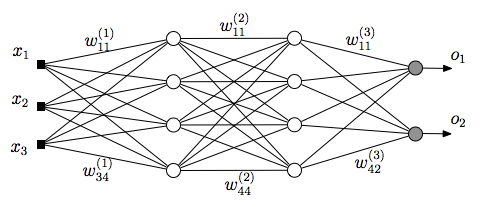
\includegraphics[scale=0.5]{img/MLP}
    \caption{Paveikslėlio pavyzdys}
    \label{img:mlp}
\end{figure}


\section{Eksperimentinio palyginimo rezultatai}
% tablesgenerator.com - converts calculators (e.g. excel) tables to LaTeX
\begin{table}[H]\footnotesize
  \centering
  \caption{Lentelės pavyzdys}
  {\begin{tabular}{|l|c|c|} \hline
    Algoritmas & $\bar{x}$ & $\sigma^{2}$ \\
    \hline
    Algoritmas A  & 1.6335    & 0.5584       \\
    Algoritmas B  & 1.7395    & 0.5647       \\
    \hline
  \end{tabular}}
  \label{tab:table example}
\end{table}

\end{document}
